\subsection{Automated Composition of Tests}
Even without a better system architecture, some of the problems of CPS design could be mitigated by making use of existing tests for layers of a system.  These tests are often,
particularly for the safety-critical system, extensive and useful;
however, they typically fail to cover the interaction of the systems
in any way.  In addition to the basic problem that the interactions
are not explored in existing tests, however, is a deeper problem:
tests do not compose.  Even within a single system, executing test
{\tt A}
followed by test {\tt B} seldom produces the desired union of behaviors
(e.g., even covering all code covered by {\tt A} or {\tt B}).  The
actions of {\tt A}
often interfere with those of {\tt B} (or vice versa): that is, some action
in {\tt A} is either illegal in a composed context, causing {\tt B} (and thus the
entire test) to become invalid, or
disables some behavior of {\tt B}, lowering test effectiveness.  The
ordering of test operations also matters: e.g., some actions in {\tt A} must be
before some actions in {\tt B} to produce interaction, while other actions
must be after some {\tt B} action.  \mycomment{Providing a way to allow for
greater composition of any set of tests, whether for a single system,
or multiple systems, would greatly enhance the utility of existing
tests produced either by human effort or by formal/automated testing
and verification methods.}  For compositions of safety-critical and
user-centric systems, and heterogeneous systems in general, it would
be highly desirable to be able to automatically produce tests that are
valid, have as little interference as possible, and maximize the sum
of behaviors from the composed tests.  The inability to compose tests
results in poorer testing, and thus more fault-prone and brittle
systems.

While complete automation of test composition, in general, is
impossible, we 
believe existing software testing algorithms, used in a  novel
way, could increase the composability of tests, even for
heterogeneous systems.  The widely known delta-debugging algorithms can
be used to manipulate tests for producing ``quick tests'' for embedded
systems \cite{icst2014}.  In this proposal, we suggest that further generalizing
delta-debugging can effectively automatically compose some (even quite heterogeneous) tests.  The key
concept is to let the delta-debugging algorithm remove portions of a
constructed \emph{hypothesis composition} to produce a test that has more
behavior than the na\"ive composition, and ideally detects a fault in
the composition of the systems \cite{tecpscompose}.

As an example of the problem, consider the following situation, a simplified generalization of testing efforts at NASA's Jet Propulsion
Laboratory, during the development of the Curiosity Mars Rover (Mars
Science Laboratory project) \cite{CFV08,ICSEDiff,AMAI}.  The file
system for the Curiosity Rover can be considered from two points of
view.  There is the low-level, embedded flash file system, implemented
as (essentially) a library in C.  There is also a higher-level
process, essentially a file catalog, through which other components of
the Curiosity software interact with the file system, and which is
directly accessed by ground operations teams controlling the rover.
The low-level file system, which interacts with the flash hardware,
was extensively tested using both model checking and random testing,
by a team of formal verification and software engineering researchers,
who also developed the file system software.  The high-level catalog
process was also tested extensively.  However, in this case the
testing was primarily performed manually by systems engineers and the Curiosity
QA team, using less formal and intensive approaches, due in part to a much
more complex but more limited specification of correctness.  Every
catalog test also tests the underlying file system, of course, but file system
tests do not test the catalog.  In practice, the two sets of
tests exist completely separately: the catalog tests as 
Python scripts to issue commands, and the file-system tests as C
programs or tools to generate tests.  This separation means that the catalog cannot benefit from
the more extensive tests produced for the low-level file system.  In
operation, some faults related to interaction of the catalog and the
file system were discovered.  We hypothesize that being able to
compose high-level catalog tests and low-level file system tests
might have detected some of these faults.

\mycomment{
One efficient way to mitigate this problem is to make use of the
existing tests for the individual systems.  These tests are often,
particularly for the safety-critical system, extensive and useful;
however, they typically fail to cover the interaction of the systems
in any way.  In addition to the basic problem that the interactions
are not explored in existing tests, however, is a deeper problem:
tests do not compose.  Even within a single system, executing test A
followed by test B seldom produces the desired union of behaviors
(e.g., even covering all code covered by A or B).  The actions of A
often interfere with those of B (or vice versa): that is, some action
in A is either illegal in a composed context, causing B (and thus the
entire test) to become invalid, or
disables some behavior of B, lowering test effectiveness.  The
ordering of test operations also matters: e.g., some actions in A must be
before some actions in B to produce interaction, while other actions
must be after B action.  Providing a way to allow for
greater composition of any set of tests, whether for a single system,
or multiple systems, would greatly enhance the utility of existing
tests produced either by human effort or by formal/automated testing
and verification methods.  For compositions of safety-critical and
user-centric systems, and heterogeneous systems in general, it would
be highly desirable to be able to automatically produce tests that are
valid, have as little interference as possible, and maximize the sum
of behaviors from the composed tests.  The inability to compose tests
results in poorer testing, and thus more fault-prone and brittle
systems.

While complete automation of test composition, in general, is
impossible, we propose a significant mitigation of the problem.  We
believe existing software testing algorithms, used in a highly novel
way, could greatly increase the composability of tests, even for
heterogeneous systems.  The widely known delta-debugging algorithms can
be used to manipulate tests for producing ``quick tests'' for embedded
systems \cite{icst2014}.  In this proposal, we suggest that further generalizing
delta-debugging can effectively automatically compose tests.  The key
concept is to let the delta-debugging algorithm remove portions of a
constructed \emph{hypothesis composition} to produce a test that has more
behavior than the na\"ive composition, and ideally detects a fault in
the composition of the systems.

As an example of the problem, consider the following situation,
derived from testing experiences of PI Groce at NASA's Jet Propulsion
Laboratory, during the development of the Curiosity Mars Rover (Mars
Science Laboratory project) \cite{CFV08,ICSEDiff,AMAI}.  The file
system for the Curiosity Rover can be considered from two points of
view.  There is the low-level, embedded flash file system, implemented
as (essentially) a library in C.  There is also a higher-level
process, essentially a file catalog, through which other components of
the Curiosity software interact with the file system, and which is
directly accessed by ground operations teams controlling the rover.
The low-level file system, which interacts with the flash hardware,
was extensively tested using both model checking and random testing,
by a team of formal verification and software engineering researchers,
who also developed the file system software.  The high-level catalog
process was also tested extensively.  However, in this case the
testing was primarily performed manually by systems engineers and the Curiosity
QA team, using less formal and intensive approaches, due in part to a
more complex but more limited specification of correctness.  Every
catalog test also tests the underlying file system, of course, but file system
tests do not test the catalog.  In current practice, the two sets of
tests exist completely separately: the catalog tests are typically
Python scripts to issue commands, and the file-system tests are C
programs.  This separation means that the catalog cannot benefit from
the more extensive tests produced for the low-level file system.  In
operation, some faults related to interaction of the catalog and the
file system were discovered.  We hypothesize that being able to
compose high-level catalog tests and low-level file system tests
properly might have detected some of these faults.

Generating effective tests for software systems is a
fundamentally difficult task: in the final analysis, most testing
problems are computationally undecidable.  This makes effective tests
extremely valuable.  Generating tests from scratch for the composition
of systems is difficult and inefficient, but determining the proper
interleaving and avoiding interference in existing tests is the kind
of tedious, error-prone task that is best solved by automated methods,
rather than left to test engineers.  Note that even in such a
motivated environment as JPL's
billion-dollar flagship Mars mission, the effort to combine the
model-checking and fuzzer generated tests for the low-level file
system and the high-level, system-engineer-devised tests for the
catalog was not even considered as an option, in the absence of
automation.}

The basic technical approach is best explained using a variation of the motivating
Mars Rover testing scenario.  Na\"ive composition of tests for the file
system and the catalog will not work.  Low-level file system tests may
include operations that change the file system state in a way that the
catalog, which has sole control of the contents of the file system in
most directories during normal rover operation, cannot handle.
Consider the composition of test {\tt A}, for the file system, and
test {\tt B} for the catalog.  Neither {\tt A+B} (composition with
{\tt A} followed by {\tt B}) nor {\tt B+A} will provide the desired
testing functionality.  If we execute {\tt A} then {\tt B}, there may be little
interaction between systems, and {\tt A} may produce an initial state
that the catalog cannot handle.  If we execute {\tt B} then {\tt A},
the much more extensive testing of the underlying flash file system
provided by {\tt A} will not impact the catalog behavior at all, resulting
in even less interaction.  How to interleave the behaviors, while
avoiding actions in {\tt A} that violate catalog constraints, is a challenge
even for engineers well-versed in both systems.  However, imagine that
we construct a new test, {\tt (A+B)}$\times k$, consisting of {\tt A}
followed by {\tt B}, repeated $k$ times.  This test will also, due to
interference (let us assume {\tt A} violates a catalog constraint) tend to
fail immediately without exposing a real fault. How can we avoid these problems?


Delta-debugging works due to the high probability that contiguous parts
of a test are related: removing \emph{chunks} of a test can
eliminate many behaviors that are irrelevant or interfering.  Given
a test {\tt a1.a2.a3.a4.a5.a6.a7.a8} that fails, delta-debugging 
might first determine if
either of {\tt a1.a2.a3.a4} or {\tt a5.a6.a7.a8} fails; if so, it
proceeds from either.  If not, it increases the granularity of
reduction, and considers candidates {\tt a3.a4.a5.a6.a7.a8}, {\tt
  a1.a2.a5.a6.a7.a8}, {\tt a1.a2.a3.a4.a7.a8}, and {\tt
  a1.a2.a3.a4.a5. a6}, until no single component of the test can be
removed without the test no longer failing.

Cause reduction \cite{icst2014,stvrcausereduce} modifies
delta-debugging to reduce tests with respect to an arbitrary property
of the test, not just failure.  For example to produce very fast
regression tests (called ``quick tests''), automated tests can be
minimized to find smaller tests that retain full code coverage.  In
past work, this approach produced highly efficient tests for
real-world systems such as Mozilla's SpiderMonkey JavaScript engine
and the YAFFS2 flash file system used in Android.

Both cause reduction and delta-debugging traditionally require as
input a test that satisfies the property of interest, e.g., a failing
test or one with certain coverage.  However, this is not necessary.
Given a test that does not fail (or provide some other useful property
of a test), cause reduction/delta-debugging defines a search, based on
removal of components, for a test that does meet the criteria.  We
propose to construct ``base'' compositions of tests (that do not provide
useful testing), and then use cause reduction to search for a test that \emph{does}
provide useful composition of the tests.  The search has a potential
to succeed because in most cases the reason composition fails is
interference, which can be avoided by removing the interfering parts
of a test, leaving a good interleaving of test actions, made possible
by the $k$ repetitions in the base.

A concrete application of our approach to the NASA Mars rover file
system testing would work as follows.  First, construct the test {\tt
  (A+B)}$\times k$ (where $k$ is at least 2, and may need to be
larger).  We can start with small $k$ and increase $k$ if the search
for a useful test fails, since the length of the initial composed test
determines the cost of cause reduction.  The multiple copies of {\tt
  (A+B)} handle the need to interleave actions from A and B, when
combined with cause reduction.  If $k$ is at least one more than the
max of the lengths of {\tt A} and {\tt B}, then there is a possibility
(though not a guarantee) for cause reduction to produce any needed
interleaving of actions: removing all but the needed actions from each
copy yields all interleavings of a single copy of {\tt A} and {\tt B}.
The extra copy is required so that the interleaving can start with
either of {\tt A} or {\tt B}.  After constructing the initial, but
usually not successful, ``composition'' {\tt (A+B)}$\times k$, our
approach applies cause reduction to {\tt (A+B)}$\times k$, searching
for a test that: 1) does not violate catalog invariants, so is a valid
test, since a core problem of composition is the creation of invalid
tests and 2) covers at least as much code as the union of code
coverage for test {\tt A} and test {\tt B}.  Alternatively, the search
can be for a test that fails for any reason other than catalog
invariant violation.  However, in some cases, both of these searches
may fail.

\mycomment{
In addition to simple search for any test satisfying a property, which
may be ineffective due to lack of guidance, a test can be ``minimized''
with the criteria that removing some part of {\tt (A+B)}$\times k$
increases coverage over the current test version.  We call this
amplification-based reduction \cite{stvrcausereduce}.  Traditional
delta-debugging and cause reduction only remove a component from a
test when this causes the test to satisfy the criteria of interest.
If the aim is to avoid interference, especially with the goal of
causing the system to fail, the delta-debugging/cause reduction
algorithms cannot discover cases where two actions, not contiguous,
must be removed: otherwise the search would be attempting to evaluate
all subsets, and hopelessly expensive.  However, in many cases, while
removing one of two interfering actions does not completely remove
interference, it does increase the desired interaction between
systems, and so increases code coverage of one or both systems.  Using
amplification-reduction, combined with allowing local minima of
non-adequate coverage \cite{ASEAdeq} the search can make progress without
completely satisfying the final goal.}

\begin{figure}
\centering
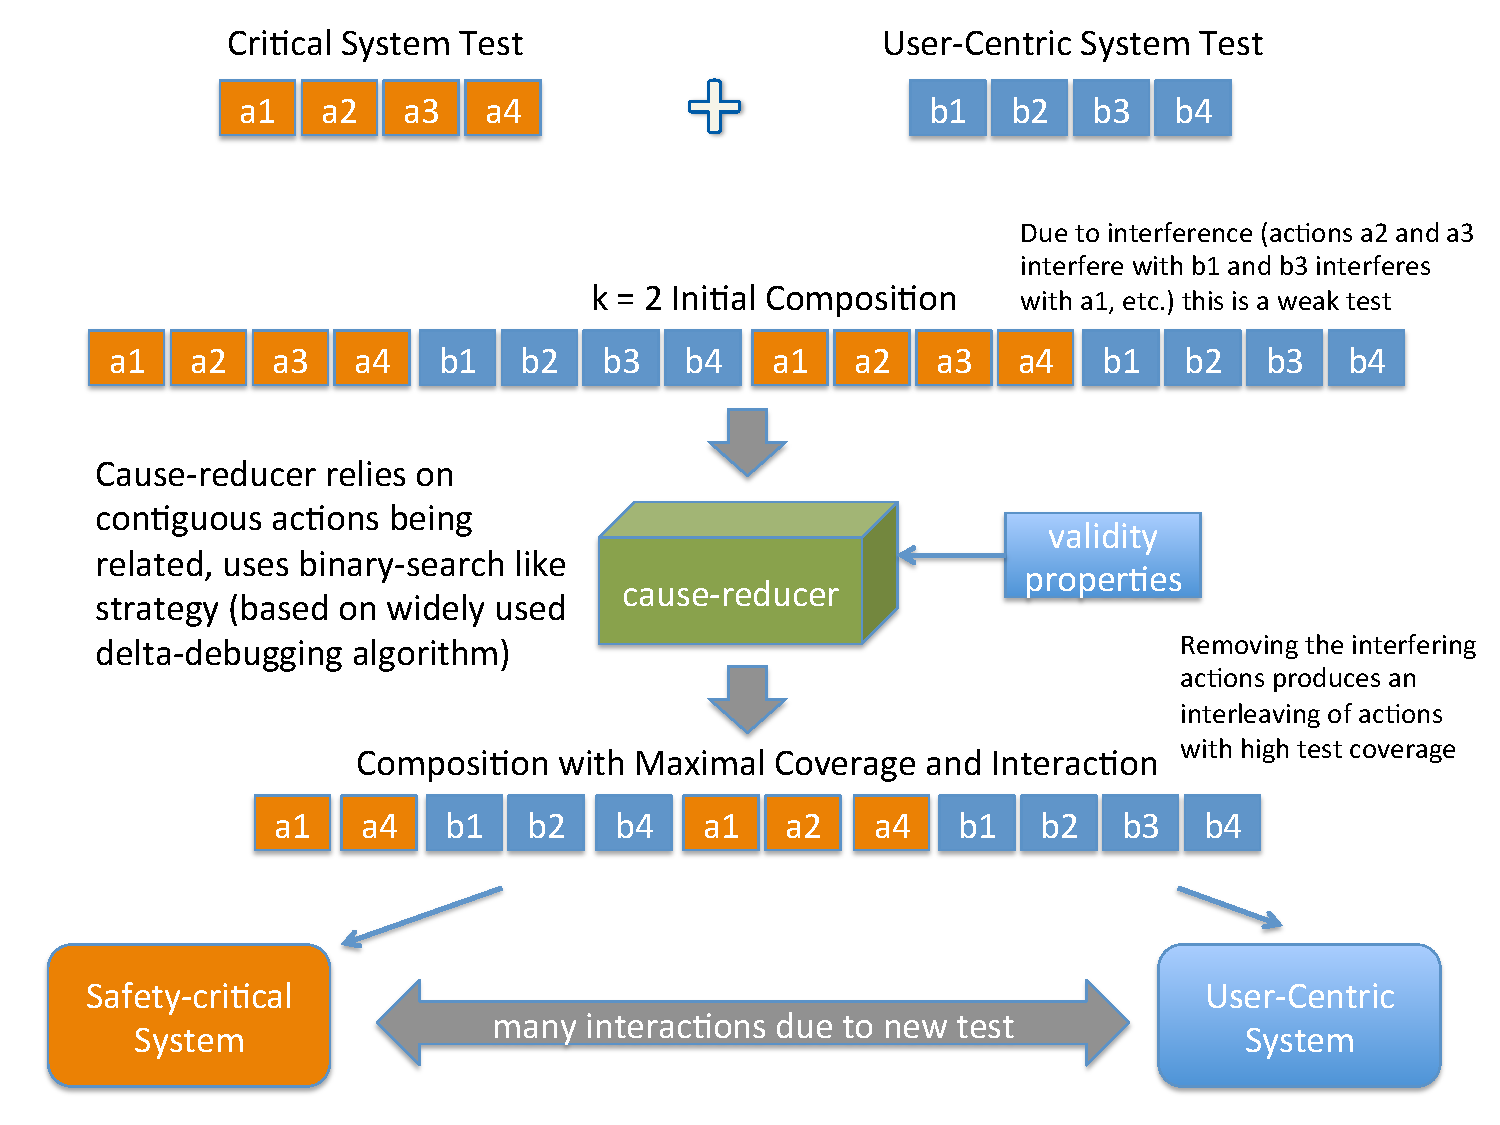
\includegraphics[width=\columnwidth]{testcomp}
\caption{Composition of heterogeneous system test cases.}
\label{fig:compose}
\end{figure}

To understand the concept, consider the simple case where {\tt A =
  a1.a2.a3.a4 and B = b1.b2.b3.b4}, with $k = 3$.  If {\tt a1}
interferes with {\tt B}, causing the catalog to fail with an invariant
violated at action {\tt b3}, then our approach can produce a test such
as: {\tt a2.a3.a4.b1.b2.b3.a1.a2.a3.a4.b1.b2.b3.b4.a1.a2.a3. a4}. Here,
{\tt a1} is removed from the copy of {\tt A} before any {\tt b3}, but
remains in the final version, from which all {\tt B} actions are
removed, because it adds new code coverage of the low-level file
system.  One {\tt b4} instance is removed, because it causes the
low-level file system code to be in a state such that the second copy
of {\tt B} exercises less code (it forces an early garbage collection
of flash blocks).  Notice that this test is not one that
delta-debugging's binary search would have proposed from the initial
test. Using gains in coverage to change the base test, we can direct
the reduction toward this high-coverage, valid, composed test without
human intervention.  Figure \ref{fig:compose} graphically shows the workflow of
automated test case composition for a different set of tests.

We implemented a simple version of our approach in TSTL \cite{tstlsttt}, and applied
it to tests (with complete code coverage) for a simple
data structure (an AVL tree).  These tests were unable to detect a
subtle, realistic, injected fault, despite covering the code. The
na\"ive composition of all tests {\tt (A+B+C+$\ldots$)} was also unable
to detect the fault, and included many invalid operations, due to
interference.  Our approach, with $k = 2$, was able to produce a test
exposing the fault in only a few seconds, by removing interfering
operations.

Because this approach suggests that test composition is essentially a
search problem, an obvious question is why we use cause
reduction/delta-debugging rather than a more traditional search-based
evolutionary or genetic algorithm approach \cite{searchtest,McMinn04search-basedsoftware,FA11}.  First, we believe that
removal of operations is the only mutation of interest in this
context: crossover or random change in test actions is likely to
introduce invalid test behavior.  Our assumption is that tests to be
composed are valid in isolation, and only nearby behaviors are of
interest (or likely to maintain single-component validity).  Second,
many search-based techniques expect access to branch distances and
other intrusive instrumentation.  This may not be feasible for
embedded systems; we can use cause reduction with instrumentation only
for user-centric code or, in the worst case, for neither system.  This
necessitates guidance by other means.

\mycomment{
\subsection{An Architecture for Testable Cyber-physical Systems}

One such means, though less well-defined at this point, is a means for expressing, via software architectural methods, the connections between domains at varying levels of abstraction.  In addition to supporting test composition (by, e.g., making explicit constraints such as those that the catalog imposes, mapped to a lower-level of abstraction), this approach would ideally enable effective testing of layers in combination with architectural models, in addition to concrete implementations.  Because complex CPS require thorough testing, given their connection to the physical world, we also aim to generally improve testability by architectural means.  For example, standardized interface descriptions could facilitate automated generation of tests at the boundaries between subsystems.


The sketch of a composition approach here is, of course, highly
incomplete. We must determine, for example, how best to choose initial
values for $k$, how to identify and make modifications to
delta-debugging that speed termination of the search or allow for
better parallelization \cite{PracMin}, and how to devise heuristics for abandoning a
failing search and using a larger $k$.  Other basic research questions
are numerous: e.g., is it best to first amplify for coverage, then
search for faults, or is this inefficient?

As an example of the kind of research question each new operation for
tests introduces, consider the fact that for some systems composition
of more than two tests may be essential to exploring interactions.
However, composing more than 4-5 tests may make cause reduction
prohibitively expensive.  How to choose only tests likely to yield
critical interactions is a novel and interesting test selection
\cite{YooHarman} problem; does composition compose?  That is, for
truly first-class tests we would expect that {\tt (A+B) + (C+D) =
  A+B+C+D} but this is far from clear in the context of test
composition, where {\tt C} and {\tt B} may have unavoidable
interference.  Another key research issue is how to extend the number
of cases where composition can succeed.  In some cases, composition of
two tests cannot proceed without ``bridging'' actions contained in
neither test.  Some bridging actions may be possible to generate
automatically, through static analysis of tests (variable renamings,
object creation and deletion, etc.), or via the same term rewriting
approach taken in normalization.  Others may require generating
random actions \cite{HamletOnly,RandFormal,DirectedSwarm,Pacheco} that cause reduction can discard if they are not needed
or are interfering.  We expect that other complexities will arise
during experimentation.
}